% !TeX root = ../../tesi.tex

To reduce the manual effort required to annotate the collected datasets and to speed up the work, an automatic labelling strategy based on Language Segment-Anything (Lang-SAM) was adopted on an offline workstation.\cite{medeiros_luca-medeiroslang-segment-anything_2026} This choice is consistent with the overall workflow adopted in this thesis, since annotation generation is computationally more suitable for a higher-resource environment than the embedded devices used for data acquisition and online inference. Lang-SAM is a zero-shot framework that combines text-guided localization and segmentation, making it possible to obtain object masks or bounding boxes directly from natural-language prompts describing the target product.

In the implemented workflow, prompts referring to dough balls or bread loaves are used to detect the products in the acquired frames. The generated bounding boxes are then manually checked for correctness and exported in a detector-compatible annotation format, in this case the COCO dataset format. This procedure provides a common labelling pipeline for both sites, significantly reduces manual annotation time, and keeps the detector-training stage consistent across the two datasets.\cite{labby_thesis_repo_2026}
\begin{figure}[h]
    \centering
    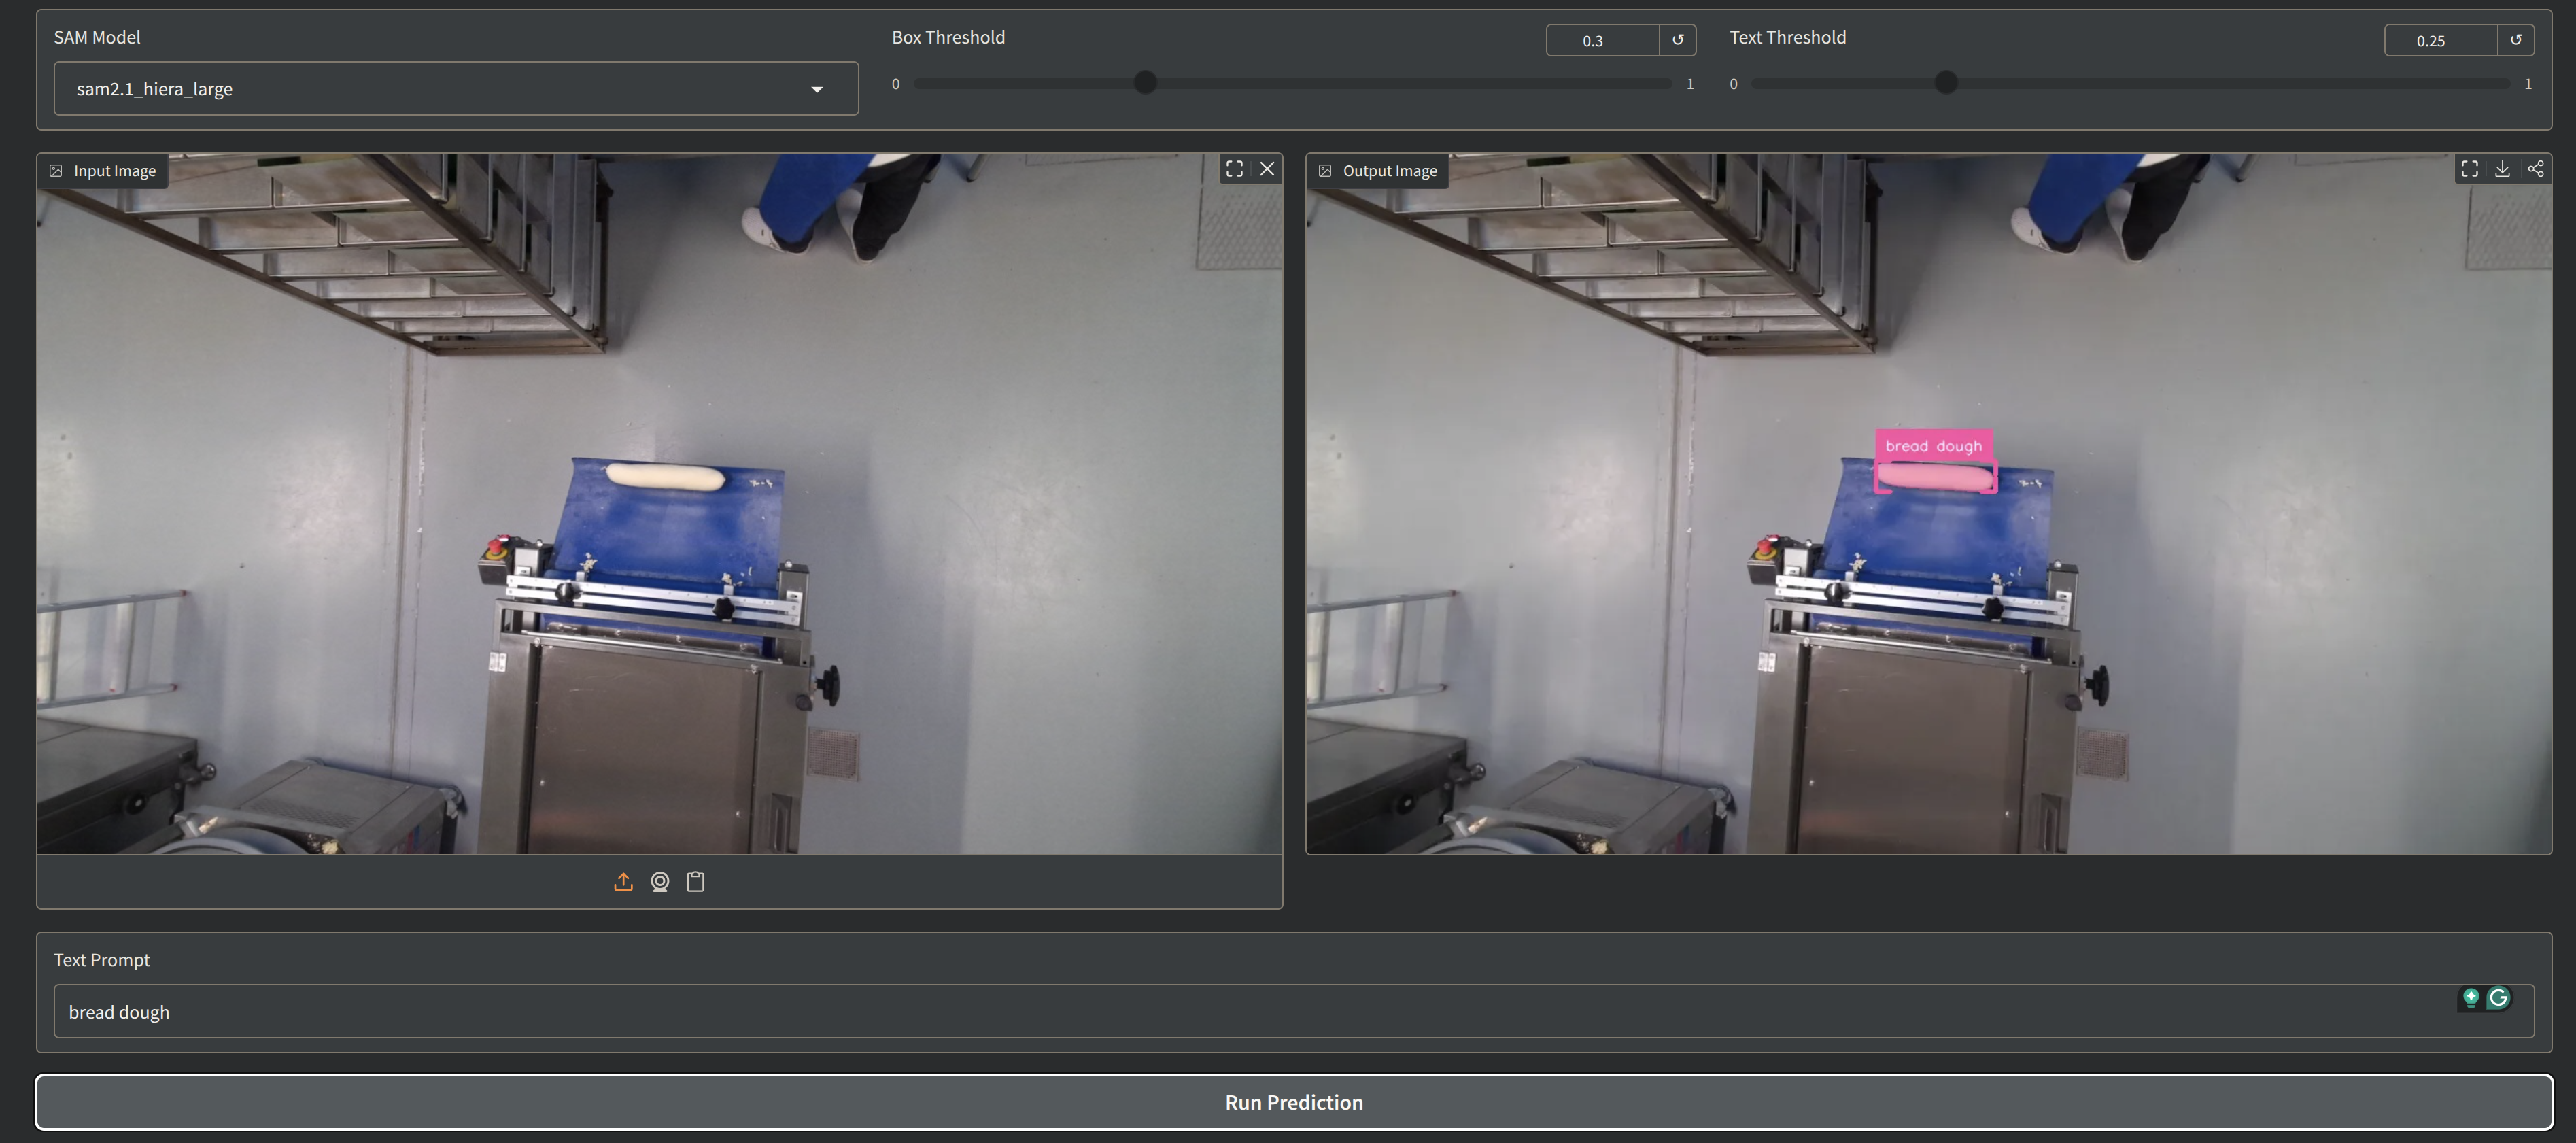
\includegraphics[width=\textwidth]{images/Useful-photos/Screenshots/Screenshot from 2026-02-23 17-16-41.png}
    \caption{Example of automatic labelling using Lang-SAM. The left image shows the original frame with a natural-language prompt describing the target product (e.g., "dough ball" or "bread loaf"). The right image displays the resulting segmentation mask and bounding box generated by Lang-SAM. This approach significantly reduces manual annotation effort while maintaining consistency across datasets.}
    \label{fig:LangSAM_labelling}
\end{figure}
